\documentclass[12pt]{article}
\usepackage[utf8]{inputenc}
\usepackage[T2A]{fontenc}
\usepackage[russian]{babel}
\usepackage{amsmath}
\usepackage{amssymb}
\usepackage{dsfont}
\usepackage[dvipsnames]{xcolor}
\usepackage{setspace}
\usepackage{multirow}
\usepackage[a4paper, outer=1.5cm, inner=1.5cm, top=1cm, bottom=1cm]{geometry}
\usepackage{graphicx}
\usepackage{skull}
\usepackage{wasysym}
\usepackage{float}
\graphicspath{{.images/}}
\usepackage{hyperref}
\hypersetup{colorlinks=true, linkcolor=blue, filecolor=magenta, urlcolor=cyan}
\usepackage[firstpage]{draftwatermark}
\SetWatermarkText{
    $\qquad\qquad\qquad\qquad\qquad$\parbox{7cm}{\begin{center}
    
\includegraphics[width = 0.08\textwidth]{lion-logo.png}\bigskip\\~\bigskip\\~\vspace{-24mm}\\~\end{center}}
}
\SetWatermarkAngle{0}
\SetWatermarkScale{1.5}
\usepackage{etoolbox}

\newtoggle{ifsolved}
\newtoggle{needhelp}
\newcounter{num}
\setcounter{num}{1}

\newcommand{\newnum}{\par\textbf{\textnumero\arabic{num}}\stepcounter{num}}
\newcommand{\sol}{\vspace{3mm}\par\textbf{Решение: }}
\newcommand{\ans}{\vspace{3mm}\par\textbf{Ответ: }}
\newcommand{\hint}{\vspace{3mm}\par\textbf{Подсказка: }}
\newcommand{\mode}[1]{
\ifstrequal{#1}{0}{\togglefalse{ifsolved}\togglefalse{needhelp}}{\ifstrequal{#1}{1}{\togglefalse{ifsolved}\toggletrue{needhelp}}{\ifstrequal{#1}{2}{\toggletrue{ifsolved}\togglefalse{needhelp}}{\toggletrue{ifsolved}\toggletrue{needhelp}}}}} %if 0 - if 1 - if 2 - else
%\newenvironment{problem}[8]{%#1, #2, #3
%\parbox{\linewidth}{\vspace{4mm}\ifstrequal{#4}{(лёгкая)}{\newnum\textbf{.}}{\newnum\textbf{*.} } \\ #5}
%\iftoggle{ifsolved}{\sol #6}{}
%\iftoggle{ifsolved}{\ans #7}{}
%\iftoggle{needhelp}{\hint #8}{}}

\newenvironment{problem}[8]{%#1, #2, #3
\parbox{\linewidth}{\vspace{5mm}\ifstrequal{#4}{(лёгкая)}{\newnum\textbf{.}}{\newnum\textbf{*.} } \\ #5}
\iftoggle{ifsolved}{\sol #6}{}

\iftoggle{ifsolved}{\parbox{\linewidth}{\ans #7}}{}
\iftoggle{needhelp}{\parbox{\linewidth}{\hint #8}}{}}

\newenvironment{mylist} %custom list
{ \begin{itemize}
    \setlength{\itemsep}{0pt}
    \setlength{\parskip}{0pt}
    \setlength{\parsep}{0pt}     }
{ \end{itemize}                  }

\newenvironment{homeass}[1]{\vspace*{-1.5cm}
\iftoggle{ifsolved}{
    \section*{\center{Решение домашнего задания к #1.}}
}{
    \section*{\center{\textcolor{Sepia}{Домашнее задание к #1}}}
} \vspace{7mm}\large}

\parindent=0pt
\pagestyle{empty}
%$\!$[\arabic{class}.\arabic{num}]
%\ifnumcomp{\value{counter}}{>}{1}{true}{false}
%\definecolor{Gray}{gray}{0.9}
%\definecolor{mypink}{RGB}{219, 48, 122}
%\newcolumntype{g}{>{\columncolor{Gray}}p{2.8cm}}

\begin{document}
\large
\mode{7}
%0 for problems without hints
%1 for problems + hints
%2 for problems + solutions + answers
%else: show all

{\centering\section*{СПИСОК ЗАДАЧ}}

{\centering\subsection*{\smallskip\\\textcolor{green}{\textbf{Полезные вещи, которые можно и нужно копипастить:}}}}

\subsection*{\textcolor{Emerald}{\textbf{Полезные шпаргалки по LaTeXу:}}}

\textbf{Пример вставки рисунка:}

\begin{minipage}{\linewidth}
    \begin{minipage}{0.54\linewidth}
    см. рисунок справа\\
    Текст к собственно пикче, примерно всегда это либо развёрнутое описание, либо большая часть решения задачи --- стремимся экономить пространство, если это можно сделать.
    \end{minipage}
    \hspace{0.05\linewidth}
    \begin{minipage}{0.4\linewidth}
    \begin{figure}[H] 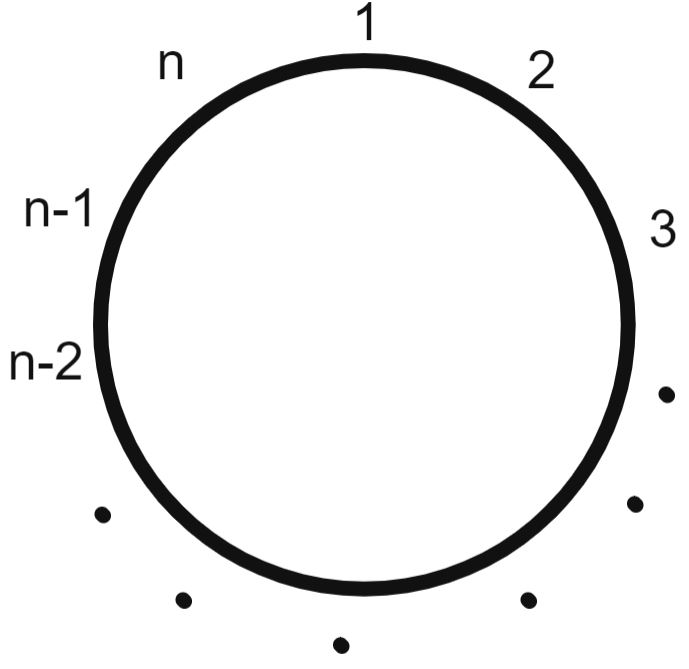
\includegraphics[width=\linewidth]{sol3} %тут поменять имя пикчи
    \end{figure}
    \end{minipage}
\end{minipage}

\textbf{Дефолтные математические знаки и символы:}\\
$\geqslant$,
$\leqslant$,
$a^{b}$,
$x_{i}$,
$\sqrt{a}$,
$\frac{a}{b}$,
$\displaystyle \frac{a}{b}$,
$\cdot$
$\;\Rightarrow\;$,
$\;\Leftrightarrow\;$,
$1{,}2$.
О промежутках:
$a\!b$,
$a\,b$,
$a\:b$,
$a\;b$,
$a\quad b$.

\textbf{Стандартные система и совокупность уравнений / неравенств:}\\
$\left\{
\begin{aligned}
f(x) &= 0 \\
g(x) &= 1
\end{aligned}\right.$

$\left[\begin{aligned}
&\left\{\begin{aligned}
f(x) &\geqslant a \\
g(x) &= b
\end{aligned}\right.\\
&\left\{\begin{aligned}
f(x) &< a \\
g(x) &= -b
\end{aligned}\right.
\end{aligned}\right.$

\subsection*{\textcolor{Emerald}{\textbf{Не математическое, но полезное:}}}
% комментарий в любом месте документа, который нигде не будет видно. Можно использовать для написания заметок-вопросов по задачам
\textbf{Пример таблицы:}

\begin{tabular}{|c|c|c|}
\hline
    $a$ & $b$ & текст
\\\hline
    $c$ & $d$ & мораль
\\\hline
\end{tabular}\\

\textbf{Отступы:} между\smallskip\\ строками\medskip\\ \textbf{Тире} --- это три дефиса.\\
\textbf{Списки:}
\begin{mylist}
\item [$\bullet$] это был пункт а
\item [2)] а это уже пункт номер 2 с изменённым заголовком
\end{mylist}

\subsection*{\textcolor{Emerald}{\textbf{Всё, неупомянутое выше (или если просто что-то не так):}}}
\begin{mylist}
\item [$\bullet$] Решение отдельных вопросов касательно ТеХа нужно искать в \href{https://www.mccme.ru/free-books/llang/newllang.pdf}{Львовском}.

\item [$\bullet$] Найти произвольный символ, который нужен, можно в \href{http://detexify.kirelabs.org/classify.html}{Detexify}.

\item [$\bullet$] Если возникли сомнения при решении, ответ практически ко всем задачам можно проверить с помощью \href{https://www.wolframalpha.com/}{WolframAlpha}.

\item [$\bullet$] Если в задаче нужно создать картинку, то лучше пока отложить эту задачу. Все графики планируется централизованно нарисовать (или перерисовать) в геогебре.

\item [\textcolor{brown}{\textbf{!!}}] Важно ставить \textcolor{red}{\textbf{$\spadesuit$}}
(или просто red) в тело задачи в случае серьёзных вопросов к решению и какой-то вопиющей лажи.

\item [\textcolor{brown}{\textbf{!!}}] Важно ставить \textcolor{olive}{\textbf{$\spadesuit$}}
(или просто olive) в тело задачи в случае не самого удачного текста и кривых отступов.
\end{mylist}

\subsection*{\textcolor{Violet}{\textbf{Комментарии:}}}% а также невидимые комментарии - так можно оставлять заметки-вопросы прямо в задаче, чтобы потом было понятно, в чём вопрос.
\begin{mylist}
\item [$\skull$] Переставлять задачи местами --- очень плохая идея.

\item [$\smiley$] При двойном клике по тексту pdf справа происходит автоматический переход к этому месту в латех-коде, а для обратного перехода можно нажать стрелку вправо (висит сверху между pdf и латех-кодом).

\item [$\smiley$] Если есть размышления, дописывать red/olive к задаче или не дописывать, то лучше всё-таки дописать.

\item [$\skull$] Самое плохое, что можно сделать --- написать в любое поле из трёх (НаписанноеРешение/ВерныйОтвет/Подсказка) только половину того, что надо, никак это не отметить, и потом пойти дальше.\\ Нужно в этот момент писать red/olive в случайном месте задачи, чтобы потом вычислить это с помощью Ctrl+F по всему документу (и это то, что потом будет делаться долго и тщательно)
\end{mylist}

\newpage
\setcounter{num}{1470}

\hypertarget{10.3}{{\centering\section*{\bigskip\\\textcolor{Blue}{\hyperlink{start2}{\textcolor{Blue}{10.3}} Тригонометрические уравнения.}\vspace{-5mm}}}}

\begin{problem}{Простейшие тригонометрические уравнения и неравенства-1.}{10.3.4}{9D}{(лёгкая)}
{Решить простейшие тригонометрические уравнения $\sin \gamma = 0$ и $\cos \theta = -1$.\\ Аккуратно записать ответ, не забыв про $2\pi n$.}
{Первое уравнение соответствует тому, что получающаяся точка имеет $y$-координату, равную 0, то есть лежит на оси абсцисс. На полуинтервале $[0; 2\pi)$ подходящих углов два: $\gamma = 0$ и $\gamma = \pi$. Не забываем про $2\pi n$: можно добавить ещё любое количество целых оборотов по окружности и получить такой же результат.\\ Таким образом, решениями уравнения $\sin\gamma = 0$ являются $\gamma = 0 + 2\pi k = 2\pi k$, $k \in \mathbb{Z}$ и $\gamma = \pi + 2\pi l$, $l \in \mathbb{Z}$. Или, что то же самое, $\gamma = \pi m$, $m \in \mathbb{Z}$.\smallskip\\
Решаем второе уравнение $\cos \theta = -1$: в данном случае получающаяся точка имеет $x$-координату, равную $-1$. Поэтому на полуинтервале $[0; 2\pi)$ подойдёт лишь одно значение $\theta = \pi$. Учитывая, что можно добавить произвольное число полных оборотов, получаем $\theta = \pi + 2\pi n$, $n \in\mathbb{Z}$.}
{Решением первого уравнения $\sin \gamma = 0$ являются $\gamma = \pi m$, $m \in \mathbb{Z}$.\\ Решением второго~--- $\cos \theta = -1$ являются $\theta = \pi + 2\pi n$, $n \in\mathbb{Z}$.}{Сначала следует найти все решения уравнения на $[0; 2\pi)$, а затем учесть возможные дополнительные обороты.}
\end{problem}

\begin{problem}{Простейшие тригонометрические уравнения и неравенства-1.}{10.3.4}{9D}{(лёгкая)}
{Решить простейшее тригонометрическое уравнение $\sin x = 0{,}5$.}
{Точка на тригонометрической окружности имеет ординату, равную $\frac12$.\\ Это табличное значение синуса: соответствующий этому значению синуса угол (в радианах) на отрезке $[-\frac{\pi}{2}; \frac{\pi}{2}]$ равен $\frac{\pi}{6}$. Согласно формулам приведения, $\sin(\pi - \alpha) = \sin\alpha$, поэтому вторым решением на полуинтервале $[0; 2\pi)$ будет $x = \pi - \frac{\pi}{6} = \frac{5\pi}{6}$.\\
Учитываем возможное добавление $2\pi n$ в силу периодичности синуса, получаем ответ: $x = \frac{\pi}{6} + 2\pi n$, $n \in \mathbb{Z}$ или $x = \frac{5\pi}{6} + 2\pi n$, $n \in \mathbb{Z}$.}
{Тригонометрическое уравнение $\sin x = 0{,}5$ имеет две бесконечных серии решений: $x = \frac{\pi}{6} + 2\pi n$, $n \in \mathbb{Z}$ или $x = \frac{5\pi}{6} + 2\pi n$, $n \in \mathbb{Z}$.}{Серий решений здесь две!}
\end{problem}

\begin{problem}{Простейшие тригонометрические уравнения и неравенства-1.}{10.3.4}{9D}{(лёгкая)}
{Решить простейшее тригонометрическое уравнение $\sin x = -\frac{\sqrt{2}}{2}$.}
{НаписанноеРешение}
{ВерныйОтвет}{Подсказка}
\end{problem}

\begin{problem}{Простейшие тригонометрические уравнения и неравенства-1.}{10.3.4}{9D}{(лёгкая)}
{Решить простейшее тригонометрическое уравнение $\cos \alpha = -0{,}5$.}
{Точка на тригонометрической окружности имеет абсциссу, равную $-\frac12$.\\ Это табличное значение косинуса: соответствующий этому значению косинуса угол (в радианах) на отрезке $[0; \pi]$ равен $\frac{2\pi}{3}$. В силу чётности косинуса $\cos(-\alpha) = \cos\alpha$, поэтому вторым решением на полуинтервале $[0; 2\pi)$ будет $\alpha = -\frac{2\pi}{3}$.\\
Учитывая возможное добавление $2\pi n$ в силу периодичности косинуса, получаем ответ: $\alpha = \pm\frac{2\pi}{3} + 2\pi n$, $n \in \mathbb{Z}$.}
{Тригонометрическое уравнение $\cos \alpha = -0{,}5$ имеет две бесконечных серии решений: $\alpha = \frac{2\pi}{3} + 2\pi n$, $n \in \mathbb{Z}$ или $\alpha = -\frac{2\pi}{3} + 2\pi n$, $n \in \mathbb{Z}$.}{Серий решений здесь две!}
\end{problem}

\begin{problem}{Простейшие тригонометрические уравнения и неравенства-1.}{10.3.4}{9D}{(лёгкая)}
{Решить простейшее тригонометрическое уравнение $\cos x = \frac{\sqrt{3}}{2}$.}
{НаписанноеРешение}
{ВерныйОтвет}{Подсказка}
\end{problem}

\begin{problem}{Простейшие тригонометрические уравнения и неравенства-1.}{10.3.4}{9D}{(лёгкая)}
{Решить уравнение $2\sin \frac{x}{2} = -\sqrt{3}$.}
{$2\sin \frac{x}{2} = -\sqrt{3} \;\Rightarrow\; \sin \frac{x}{2} = -\frac{\sqrt{3}}{2}$. Решаем простейшее тригонометрическое уравнение относительно $\frac x2$. Значение $-\frac{\sqrt{3}}{2}$ является табличным значением синуса, получаем, что $\frac x2 = -\frac{\pi}{3} + 2\pi n$, $n \in \mathbb{Z}\,$ или $\,\frac x2 = -\frac{2\pi}{3} + 2\pi n$, $n \in \mathbb{Z}$.\\
Отсюда имеем $x = -\frac{2\pi}{3} + 4\pi n$, $n \in \mathbb{Z}\,$ или $\,x = -\frac{4\pi}{3} + 4\pi n$, $n \in \mathbb{Z}$.}
{$x = -\frac{2\pi}{3} + 4\pi n$, $n \in \mathbb{Z}\,$ или $\,x = -\frac{4\pi}{3} + 4\pi n$, $n \in \mathbb{Z}$.}{Данное тригонометрическое уравнение сводится к простейшему.}
\end{problem}

\begin{problem}{Простейшие тригонометрические уравнения и неравенства-1.}{10.3.4}{9D}{(лёгкая)}
{Решить простейшее тригонометрическое уравнение $0{,}4\sin (x + \frac{\pi}{8}) = \frac{\sqrt{2}}{5}$.}
{НаписанноеРешение}
{ВерныйОтвет}{Подсказка}
\end{problem}

\begin{problem}{Методы решения тригонометрических уравнений-1.}{10.3.6}{9D}{(лёгкая)}
{Решить тригонометрическое уравнение $\,\sin (\beta + \frac{\pi}{12}) = \frac{\sqrt{3}}{2}$.}
{Соответствующая углу $\beta + \frac{\pi}{12}$ точка на тригонометрической окружности имеет ординату, равную $\frac{\sqrt{3}}{2}$. Это табличное значение: на отрезке $[-\frac{\pi}{2}; \frac{\pi}{2}]$ подходящий угол равен $\frac{\pi}{3}$. Это означает, что $\beta + \frac{\pi}{12} = \frac{\pi}{3} \;\Rightarrow\; \beta = \frac{\pi}{3} - \frac{\pi}{12} = \frac{\pi}{4}$.\smallskip\\ В силу формулы приведения, $\beta + \frac{\pi}{12}$ также может быть равно $\pi - \frac{\pi}{3} = \frac{2\pi}{3}$, откуда $\beta = \frac{2\pi}{3} - \frac{\pi}{12} = \frac{7\pi}{12}$. Других подходящих углов на полуинтервале $[0; 2\pi)$ нет, функция $f(x) = \sin(x + \frac{\pi}{12})$ является периодической с периодом $2\pi$, поэтому всего есть две серии решений: $\beta = \frac{\pi}{4} + 2\pi n$, $n \in \mathbb{Z}\,$ или $\beta = \frac{7\pi}{12} + 2\pi n$, $n \in \mathbb{Z}$.}
{$\beta = \frac{\pi}{4} + 2\pi n$, $n \in \mathbb{Z}\,$ или $\beta = \frac{7\pi}{12} + 2\pi n$, $n \in \mathbb{Z}$.}{Серий решений здесь две.\\ Также не стоит забывать, что под синусом ещё стоит $\frac{\pi}{12}$.}
\end{problem}

\begin{problem}{Простейшие тригонометрические уравнения и неравенства-1.}{10.3.4}{9D}{(лёгкая)}
{Решить простейшее тригонометрическое уравнение $2\cos (x - \frac{\pi}{3}) = 1$.}
{НаписанноеРешение}
{ВерныйОтвет}{Подсказка}
\end{problem}

\begin{problem}{Простейшие тригонометрические уравнения и неравенства-1.}{10.3.4}{9D}{(лёгкая)}
{Решить простейшее тригонометрическое уравнение $2\cos (x - \frac{5\pi}{12}) = \sqrt{2}$.}
{Поделив обе части данного уравнения на 2, получим простейшее тригонометрическое уравнение относительно $x - \frac{5\pi}{12}$: $\;\cos (x - \frac{5\pi}{12}) = \frac{\sqrt{2}}{2}$, откуда имеем\\ $x - \frac{5\pi}{12} = \pm\frac{\pi}{4} + 2\pi n$, $n\in\mathbb{Z}$. Отсюда получаем две серии решений этого уравнения:\\ $x = \frac{\pi}{4} + \frac{5\pi}{12} + 2\pi n = \frac{2\pi}{3} + 2\pi n$, $n\in\mathbb{Z}\;$ и $\;x = -\frac{\pi}{4} + \frac{5\pi}{12} + 2\pi n = \frac{\pi}{6} + 2\pi n$, $n\in\mathbb{Z}$.}
{Данное уравнение имеет две серии решений: $x = \frac{2\pi}{3} + 2\pi n$, $n\in\mathbb{Z}\,$ и $x = \frac{\pi}{6} + 2\pi n$, $n\in\mathbb{Z}$.}{Это табличное значение косинуса~--- получится две серии решений.}
\end{problem}

\begin{problem}{Простейшие тригонометрические уравнения и неравенства-1.}{10.3.4}{9D}{(лёгкая)}
{Решить уравнение $\cos 5x = \frac{1}{\sqrt{2}}$.}
{$\cos 5x = \frac{1}{\sqrt{2}} \;\Rightarrow\; \cos 5x = \frac{\sqrt{2}}{2}$. Решаем простейшее тригонометрическое уравнение относительно $5x$. Значение $\frac{\sqrt{2}}{2}$ является табличным значением косинуса, получаем, что $5x = \frac{\pi}{4} + 2\pi n$, $n \in \mathbb{Z}\,$ или $\,5x = -\frac{\pi}{4} + 2\pi n$, $n \in \mathbb{Z}$.\\
Отсюда имеем $x = \frac{\pi}{20} + \frac{2\pi n}{5}$, $n \in \mathbb{Z}\,$ или $\,x = -\frac{\pi}{20} + \frac{2\pi n}{5}$, $n \in \mathbb{Z}$, или, что то же самое, $\vphantom{\Bigr(} x = \frac{\pi}{20} + 2\pi n$, $x = \frac{7\pi}{20} + 2\pi n$, $x = \frac{9\pi}{20} + 2\pi n$, $x = \frac{3\pi}{4} + 2\pi n$, $x = \frac{17\pi}{20} + 2\pi n$, $x = \frac{23\pi}{20} + 2\pi n$, $x = \frac{5\pi}{4} + 2\pi n$, $x = \frac{31\pi}{20} + 2\pi n$, $x = \frac{33\pi}{20} + 2\pi n$, $x = \frac{39\pi}{20} + 2\pi n$, $n \in \mathbb{Z}$.

{\centering (то есть, всего есть 10 серий решений).

}}
{Решениями уравнения $\cos 5x = \frac{1}{\sqrt{2}}$ являются $x = \pm\frac{\pi}{20} + \frac{2\pi n}{5}$, $n \in \mathbb{Z}$.}{Данное тригонометрическое уравнение сводится к простейшему.}
\end{problem}

\begin{problem}{Простейшие тригонометрические уравнения и неравенства-1.}{10.3.4}{9D}{(лёгкая)}
{Решить простейшее тригонометрическое уравнение $\sin \beta = 0{,}7$.\\ С помощью калькулятора вычислить ответ в градусах с точностью до третьего знака после запятой.}
{Решением простейшего тригонометрического уравнения $\sin x = a$ является $x = (-1)^n \arcsin(a) + \pi n$, $n \in \mathbb{Z}$. Поэтому есть две бесконечных серии решений: $\beta = \arcsin(0{,}7) + 2\pi n$, $n \in \mathbb{Z}$, и $\beta = \pi - \arcsin(0{,}7) + 2\pi n$, $n \in \mathbb{Z}$.\\
Вычисляя ответ с помощью калькулятора, получаем $\arcsin(0{,}7) \approx 44{,}427^{\circ}$.\\ Таким образом, на полуинтервале $[0; 360)$ подходящими значениями являются $\beta \approx 44{,}427^{\circ}$ и $\beta \approx 180^{\circ} - 44{,}427^{\circ} = 135{,}573^{\circ}$.}
{Решениями уравнения $\sin \beta = 0{,}7$ являются $\beta = \arcsin(0{,}7) + 2\pi n$, $n \in \mathbb{Z}$, и $\beta = \pi - \arcsin(0{,}7) + 2\pi n$, $n \in \mathbb{Z}$. Соответственно, значения углов на $[0; 360)$ получаются равными примерно $44{,}427^{\circ}$ и $135{,}573^{\circ}$.\\
\textit{Комментарий:} углы отличаются от табличных углов $45^{\circ}$ и $135^{\circ}$ всего на полградуса. Это связано с тем, что $0{,}7$ весьма близко к $\sin(45^{\circ}) = \frac{\sqrt{2}}{2} \approx 0{,}707$.}{Ответ можно и нужно давать с невычисленным арксинусом.}
\end{problem}

\begin{problem}{Простейшие тригонометрические уравнения и неравенства-1.}{10.3.4}{9D}{(лёгкая)}
{Решить простейшее тригонометрическое уравнение $\cos \beta = -0{,}02$.\\ С помощью калькулятора вычислить ответ в градусах с точностью до третьего знака после запятой.}
{Решением простейшего тригонометрического уравнения $\cos x = b$ является $x = \pm\arccos(b) + 2\pi n$, $n \in \mathbb{Z}$. Поэтому есть две бесконечных серии решений: $\beta = \arccos(-0{,}02) + 2\pi n$, $n \in \mathbb{Z}$, и $\beta = \arccos(-0{,}02) + 2\pi n$, $n \in \mathbb{Z}$.\\
Вычисляя ответ с помощью калькулятора, получаем $\arccos(-0{,}02) \approx 91{,}146^{\circ}$.\\ Таким образом, на полуинтервале $[0; 360)$ подходящими значениями являются $\beta \approx 91{,}146^{\circ}$ и $\beta \approx 360^{\circ} - 91{,}146^{\circ} = 268{,}854^{\circ}$.}
{Решениями уравнения $\cos \beta = -0{,}02$ являются $\beta = \pm\arccos(-0{,}02) + 2\pi n$, $n \in \mathbb{Z}$. Соответственно, значения углов на $[0; 360)$ получаются равными примерно $91{,}146^{\circ}$ и $268{,}854^{\circ}$.\\
\textit{Комментарий:} углы практически не отличаются от табличных углов $90^{\circ}$ и $270^{\circ}$. Это связано с тем, что $-0{,}02$ очень близко к $\cos(90^{\circ}) = 0$.}{Ответ можно и нужно давать с невычисленным арккосинусом.}
\end{problem}

\begin{problem}{Простейшие тригонометрические уравнения и неравенства-1.}{10.3.4}{9D}{(лёгкая)}
{Решить простейшее тригонометрическое уравнение $\tg \beta = 1$.}
{Решением простейшего тригонометрического уравнения $\tg x = c$ является $x = \arctg(c) + \pi n$, $n \in \mathbb{Z}$. Однако, тангенс равный 1~--- табличное значение (действительно, если отношение катетов равно 1, то катеты равны, возникает равнобедренный треугольник). Поэтому получаем (без калькулятора), что $\arctg(1) = \frac{\pi}{4}$. Таким образом, $\beta = \frac{\pi}{4} + \pi n$, $n \in \mathbb{Z}$.}
{Решением уравнения $\tg \beta = 1$ является $\beta = \frac{\pi}{4} + \pi n$, $n \in \mathbb{Z}$.}{Это табличное значение тангенса, калькулятор тут не нужен.}
\end{problem}

\begin{problem}{Простейшие тригонометрические уравнения и неравенства-1.}{10.3.4}{9D}{(лёгкая)}
{Решить простейшее тригонометрическое уравнение $\tg \beta = -\sqrt{3}$.}
{НаписанноеРешение}
{ВерныйОтвет}{Подсказка}
\end{problem}

\begin{problem}{Простейшие тригонометрические уравнения и неравенства-1.}{10.3.4}{9D}{(лёгкая)}
{Решить простейшее тригонометрическое уравнение $\tg x = \frac{\sqrt{3}}{3}$.}
{НаписанноеРешение}
{ВерныйОтвет}{Подсказка}
\end{problem}

\begin{problem}{Простейшие тригонометрические уравнения и неравенства-1.}{10.3.4}{9D}{(лёгкая)}
{Решить простейшее тригонометрическое уравнение $\ctg \beta = 0$.}
{НаписанноеРешение}
{ВерныйОтвет}{Подсказка}
\end{problem}

\begin{problem}{Простейшие тригонометрические уравнения и неравенства-1.}{10.3.4}{9D}{(лёгкая)}
{Решить простейшее тригонометрическое уравнение $\ctg \beta = \frac{\sqrt{3}}{3}$.}
{Решением простейшего тригонометрического уравнения $\ctg x = d$ является $x = \arcctg(d) + \pi n$, $n \in \mathbb{Z}$. Однако, котангенс равный $\frac{\sqrt{3}}{3}$~--- табличное значение, получаем $\arcctg\left(\frac{\sqrt{3}}{3}\right) = \frac{\pi}{3}$. Таким образом, $\beta = \frac{\pi}{3} + \pi n$, $n \in \mathbb{Z}$.\vspace{-3mm}}
{Решением уравнения $\ctg \beta = \frac{\sqrt{3}}{3}$ является $\beta = \frac{\pi}{3} + \pi n$, $n \in \mathbb{Z}$.}{Это табличное значение котангенса, калькулятор тут не нужен.}
\end{problem}

\begin{problem}{Простейшие тригонометрические уравнения и неравенства-1.}{10.3.4}{9D}{(лёгкая)}
{Решить простейшее тригонометрическое уравнение $\ctg \beta = -1$.}
{Решаем простейшее тригонометрическое уравнение, $-1$~--- табличное значение котангенса. Получаем, что $\beta = -\frac{\pi}{4} + \pi n$, $n \in \mathbb{Z}$. Таким образом, есть две серии решений: $\beta = -\frac{\pi}{4} + 2\pi n$, $n \in \mathbb{Z}\,$ и $\,\beta = \frac{3\pi}{4} + 2\pi n$, $n \in \mathbb{Z}$.}
{$\beta = -\frac{\pi}{4} + 2\pi n$, $n \in \mathbb{Z}\,$ или $\,\beta = \frac{3\pi}{4} + 2\pi n$, $n \in \mathbb{Z}$.}{Это табличное значение котангенса.}
\end{problem}

\begin{problem}{Простейшие тригонометрические уравнения и неравенства-1.}{10.3.4}{9D}{(лёгкая)}
{Решить простейшее тригонометрическое уравнение $4\tg (x - 1) + 4 = 0$.}
{НаписанноеРешение}
{ВерныйОтвет}{Подсказка}
\end{problem}

\begin{problem}{Простейшие тригонометрические уравнения и неравенства-1.}{10.3.4}{9D}{(лёгкая)}
{Решить тригонометрическое уравнение $\sqrt{3}\tg \beta = 1$.}
{$\sqrt{3}\tg \beta = 1 \;\Rightarrow\; \tg \beta = \frac{\sqrt{3}}{3}$. Решаем простейшее тригонометрическое уравнение. Значение $\frac{\sqrt{3}}{3}$ является табличным значением тангенса, поэтому получаем, что $\beta = \frac{\pi}{6} + \pi n$, $n \in \mathbb{Z}$. Таким  образом, есть две серии решений:\\ $\beta = \frac{\pi}{6} + 2\pi n$, $n \in \mathbb{Z}$, и $\beta = \frac{7\pi}{6} + 2\pi n$, $n \in \mathbb{Z}$.}
{Решениями являются $\beta = \frac{\pi}{6} + 2\pi n$, $n \in \mathbb{Z}$, и $\beta = \frac{7\pi}{6} + 2\pi n$, $n \in \mathbb{Z}$.}{Данное тригонометрическое уравнение сводится к простейшему.}
\end{problem}

\begin{problem}{Простейшие тригонометрические уравнения и неравенства-1.}{10.3.4}{9D}{(лёгкая)}
{Решить простейшее тригонометрическое уравнение $\ctg (2x + \frac{\pi}{4}) - \sqrt{3} = 0$.}
{НаписанноеРешение}
{ВерныйОтвет}{Подсказка}
\end{problem}

\begin{problem}{Простейшие тригонометрические уравнения и неравенства-1.}{10.3.4}{9D}{(лёгкая)}
{Решить простейшее тригонометрическое уравнение $\ctg (\frac{\pi}{12} - 3x) = 1$.}
{$\ctg\alpha = 1$~--- табличное значение котангенса ($\cos\alpha = \sin\alpha$).\\ Поэтому при решении уравнения получается, что $\frac{\pi}{12} - 3x = \frac{\pi}{4} + \pi n$, $\,n\in\mathbb{Z}$.\\ Отсюда $\,3x = \frac{\pi}{12} - \frac{\pi}{4} - \pi n = -\frac{\pi}{6} + \pi k$, $\,n, k\in\mathbb{Z}$. Итого, $x = -\frac{\pi}{18} + \frac{\pi k}{3}$, $\,k\in\mathbb{Z}$.}
{Решениями данного уравнения являются $x = -\frac{\pi}{18} + \frac{\pi k}{3}$, $\,k\in\mathbb{Z}$.}{Это табличное значение котангенса.}
\end{problem}

\begin{problem}{Методы решения тригонометрических уравнений-1.}{10.3.6}{9D}{(лёгкая)}
{a) Решить уравнение $\displaystyle \frac{2\sin^{2} x - \sin x}{2\cos x - \sqrt{3}} = 0$.
\\b) Найти все корни этого уравнения, принадлежащие отрезку $\displaystyle\left[\frac{3\pi}{2}; 3\pi\right]$}
{НаписанноеРешение}
{ВерныйОтвет}{Подсказка}
\end{problem}

\begin{problem}{Методы решения тригонометрических уравнений-1.}{10.3.6}{9D}{(лёгкая)}
{Решить уравнение $\displaystyle (\tg^{2} x - 1)\sqrt{13\cos x} = 0$.}
{НаписанноеРешение}
{ВерныйОтвет}{Подсказка}
\end{problem}

\begin{problem}{Методы решения тригонометрических уравнений-1.}{10.3.6}{9D red 10.4.7?}{(лёгкая)}
{Изобразить на тригонометрической окружности точки, являющиеся решением уравнения $\,\displaystyle \frac{\cos 3x}{\cos x} = 0$.}
{Воспользуемся формулой косинуса тройного угла и подставим полученное в числитель: $\cos 3x = 4\cos^3 x - 3\cos x \;\Rightarrow\; \displaystyle \frac{4\cos^3 x - 3\cos x}{\cos x} = 0 \; \Rightarrow $ \\ $\Rightarrow\; \displaystyle \frac{\cos x \cdot (4\cos^2 x - 3)}{\cos x} = 0 \;\Leftrightarrow\; \left\{\begin{aligned}
\cos x \neq 0\!\!\!&\\
4\cos^2 x - 3 &= 0
\end{aligned}\right. \;\Leftrightarrow\; \left\{\begin{aligned}
\cos x &\neq 0\\
\cos x &= \pm\frac{\sqrt{3}}{2}
\end{aligned}\right. \;\Leftrightarrow\;$ \\$\cos x = \pm\frac{\sqrt{3}}{2} \;\Leftrightarrow\; x = \pm\frac{\pi}{6} + \pi n$, $n\in\mathbb{Z}$. Это и есть ответ.\\
Можно решать и иначе: $\,\displaystyle \frac{\cos 3x}{\cos x} = 0 \;\Leftrightarrow\; \left\{\begin{aligned}
    \cos x &\neq 0\\
    \cos 3x &= 0
    \end{aligned}\right. \;\Leftrightarrow\; \left\{\begin{aligned}
    x &\neq \frac{\pi}{2} + \pi k,\, k\in\mathbb{Z}\\
    3x &= \frac{\pi}{2} + \pi n,\, n\in\mathbb{Z}
    \end{aligned}\right. \;\Leftrightarrow$
\vspace{-4mm}\\\begin{minipage}{\linewidth}
    \begin{minipage}{0.54\linewidth}
    $\,\displaystyle \;\Leftrightarrow\; \left\{\begin{aligned}
    x &\neq \frac{\pi(3 + 6k)}{6},\, k\in\mathbb{Z}\\
    x &= \frac{\pi(1 + 2n)}{6},\, n\in\mathbb{Z}.
    \end{aligned}\right.$\bigskip\\
    То есть точки идут с периодом $\frac{\pi}{3}$, но каждая третья (номер которой делится на 3) выбрасывается, так как мы не можем делить на 0.\medskip\\
    Ситуация на полуинтервале $[0; 2\pi)$ изображена на рисунке справа.
    \end{minipage}
    \hspace{0.04\linewidth}
    \begin{minipage}{0.4\linewidth}\begin{figure}[H] 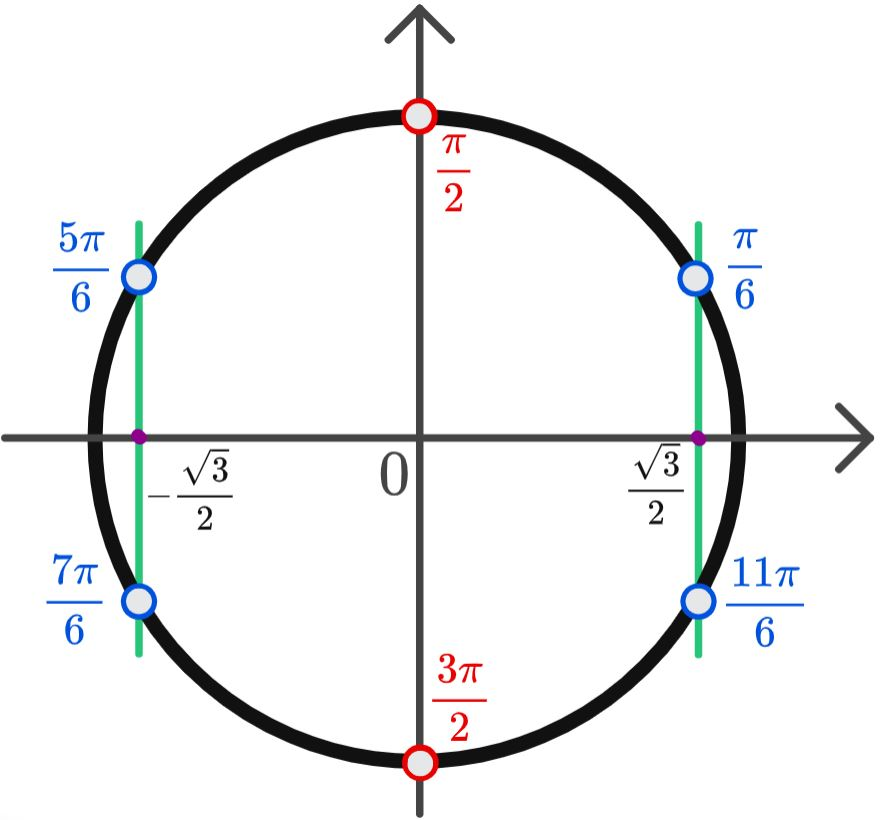
\includegraphics[width=\linewidth]{sol45}\end{figure}\end{minipage}
\end{minipage}\vspace{-5mm}\\}
{Решением уравнения $\,\displaystyle \frac{\cos 3x}{\cos x} = 0$ являются точки $x = \pm\frac{\pi}{6} + \pi n$, $n\in\mathbb{Z}$.}{Главное~--- не забыть учесть, что знаменатель дроби не равен нулю.}
\end{problem}

\begin{problem}{Методы решения тригонометрических уравнений-1.}{10.3.6}{9D}{(лёгкая)}
{Решить уравнение $\,\displaystyle \frac{1}{\sin^{2} x} - \frac{3}{\sin x} + 2 = 0$.}
{Очевидно, что в данном случае напрашивается замена $s = \sin x$.\\ Сделаем её и решим полученное рациональное уравнение относительно $s$:\\
$\displaystyle \frac{1}{s^2} - \frac{3}{s} + 2 = 0 \;\Leftrightarrow\; \frac{1 - 3s + 2s^2}{s^2} = 0 \;\Rightarrow\; 2s^2 - 3s + 1 = 0 \;\Leftrightarrow\; (s - 1)(2s - 1) = 0$.\smallskip\\
Итого, данное уравнение на $s$ имеет два решения: $s = 1$ или $s = \frac12$.\\ Теперь делаем обратную замену и решаем каждое уравнение отдельно:\\ $\left[\begin{aligned}
s &= 1\\
s &= \frac12
\end{aligned}\right. \;\Leftrightarrow\;
\left[\begin{aligned}
\sin x &= 1\\
\sin x &= \frac12
\end{aligned}\right. \;\Leftrightarrow\;
\left[\begin{aligned}
x &= \frac{\pi}{2} + 2\pi n, \,n \in\mathbb{Z}\\
x &= \arcsin\left(\tfrac12\right) + 2\pi n, \,n \in\mathbb{Z}\\
x &= \pi - \arcsin\left(\tfrac12\right) + 2\pi n, \,n \in\mathbb{Z}
\end{aligned}\right.$\\
Синус, равный $\frac12$~--- табличное значение. Поэтому в итоге получаем\\ $\left[\begin{aligned}
x &= \frac{\pi}{2} + 2\pi n, \,n \in\mathbb{Z}\\
x &= \frac{\pi}{6} + 2\pi n, \,n \in\mathbb{Z}\\
x &= \frac{5\pi}{6} + 2\pi n, \,n \in\mathbb{Z}
\end{aligned}\right.$}
{Уравнение $\,\displaystyle\frac{1}{\sin^{2} x} - \frac{3}{\sin x} + 2 = 0$ имеет 3 серии решений:\\ $x = \frac{\pi}{2} + 2\pi n, \,n \in\mathbb{Z},\,$ $x = \frac{\pi}{6} + 2\pi n, \,n \in\mathbb{Z},\,$ и $\,x = \frac{5\pi}{6} + 2\pi n, \,n \in\mathbb{Z}$.}{Сделай замену.}
\end{problem}

\begin{problem}{Методы решения тригонометрических уравнений-1.}{10.3.6}{9D}{(лёгкая)}
{a) Решить уравнение $\cos 2x - 3\cos x + 2 = 0$.
\\b) Найти все корни этого уравнения, принадлежащие отрезку $\displaystyle \left[-4\pi;\, -\frac{5\pi}{2}\right]$.}
{Используем формулу для косинуса двойного угла, причём выразим его через $\cos x$, так как он уже есть в нашем выражении, получаем уравнение $2\cos^2 x - 1 - 3\cos x + 2 = 0 \;\Rightarrow\; 2\cos^2 x - 3\cos x + 1 = 0$. Делаем замену $y = \cos x$:\\
$2y^2 - 3y + 1 = 0 \;\Rightarrow\; (2y - 1)(y - 1) = 0 \;\Rightarrow\; y = 1$, $\,y = \frac12$.\\ 
\vspace{-7mm}\\\begin{minipage}{\linewidth}
    \begin{minipage}{0.56\linewidth}
    Таким образом, $\,\left[
    \begin{aligned}
    y &= 1\\
    y &= \frac12
    \end{aligned}\right. \;\Leftrightarrow\;
    \left[
    \begin{aligned}
    \cos x &= 1\\
    \cos x &= \frac12
    \end{aligned}\right. \;\Leftrightarrow$\smallskip\\ $\Leftrightarrow\;\left[
    \begin{aligned}
    x &= 2\pi n,\; n\in\mathbb{Z}\\
    x &= \pm\frac{\pi}{3} + 2\pi n,\; n\in\mathbb{Z}.
    \end{aligned}\right.$\bigskip\\
    Уравнение решено. Отберём корни.\smallskip\\
    Интересующий нас отрезок изображён на\\ рисунке справа. Подходящими корнями, \\таким образом, являются $x = -4\pi$ и $-\frac{11\pi}{3}$.
    \end{minipage}
    \hspace{0.04\linewidth}
    \begin{minipage}{0.39\linewidth}\begin{figure}[H] 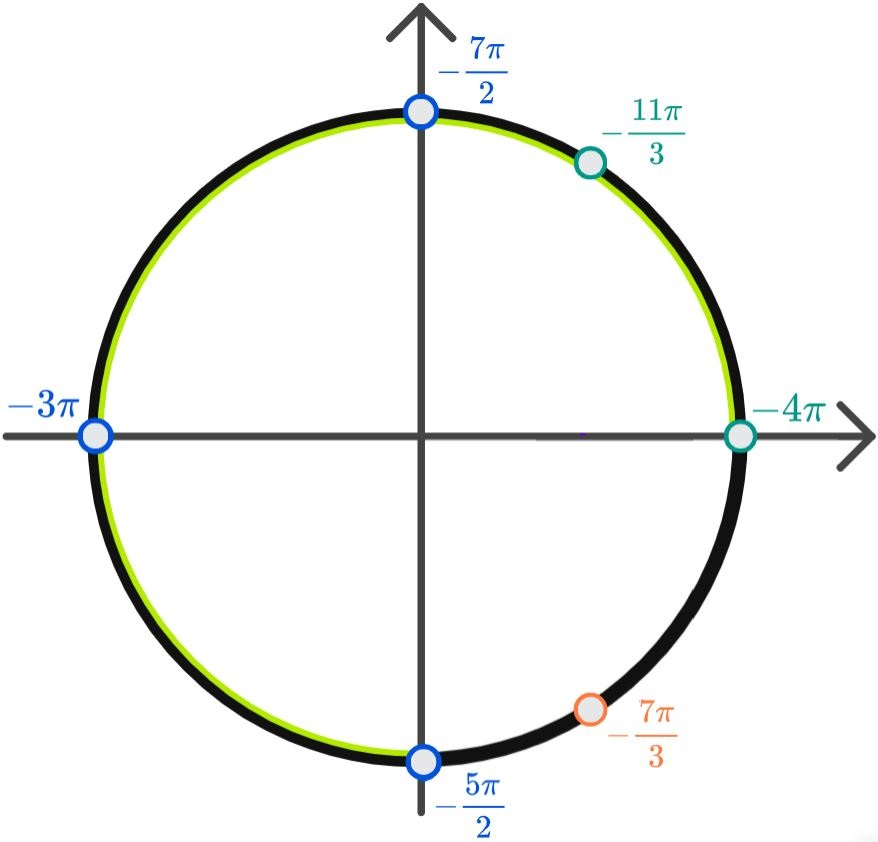
\includegraphics[width=\linewidth]{sol51}\end{figure}\end{minipage}
\end{minipage}}
{a) Решениями являются $x = 2\pi n,\; n\in\mathbb{Z}\,$ и $\,x = \pm\frac{\pi}{3} + 2\pi n,\; n\in\mathbb{Z}$.\\
~\hspace*{1.65cm} b) На отрезке $\left[-4\pi;\, -\frac{5\pi}{2}\right]$ находятся два корня: $x = -4\pi\,$ и $\,x = -\frac{11\pi}{3}$.}{Сделать замену, свести к решению простейших уравнений.}
\end{problem}

\begin{problem}{Методы решения тригонометрических уравнений-1.}{10.3.6}{9D}{(лёгкая)}
{a) Решить уравнение $\cos 2x + \sin^2 x = 0{,}75$.\\
b) Найти все корни этого уравнения, принадлежащие отрезку $\displaystyle \left[-\pi;\, \frac{\pi}{2}\right]$.}
{Используем формулу для косинуса двойного угла, причём выразим его через $\sin x$, так как он уже есть в нашем выражении, получаем уравнение $1 - 2\sin^2 x + \sin^2 x = 0{,}75 \;\Rightarrow\; \sin^2 x = \frac14$. 
\vspace{-7mm}\\\begin{minipage}{\linewidth}
    \begin{minipage}{0.56\linewidth}
    Получаем, что или $\sin x = \frac12$, или $\sin x = -\frac12$, откуда $x = \pm\frac{\pi}{6} + \pi n$, $n\in\mathbb{Z}$.\vspace{2mm}\bigskip\\ 
    Уравнение решено. Отберём корни.\medskip\\
    Интересующий нас отрезок изображён на\\ рисунке справа (здесь изображены углы от $-\frac{3\pi}{2}$ до $\frac{\pi}{2}$). Подходящими корнями, таким \\образом, являются $x = -\frac{5\pi}{6}$, $x = -\frac{\pi}{6}$ и $x = \frac{\pi}{6}$.
    \end{minipage}
    \hspace{0.04\linewidth}
    \begin{minipage}{0.39\linewidth}\begin{figure}[H] 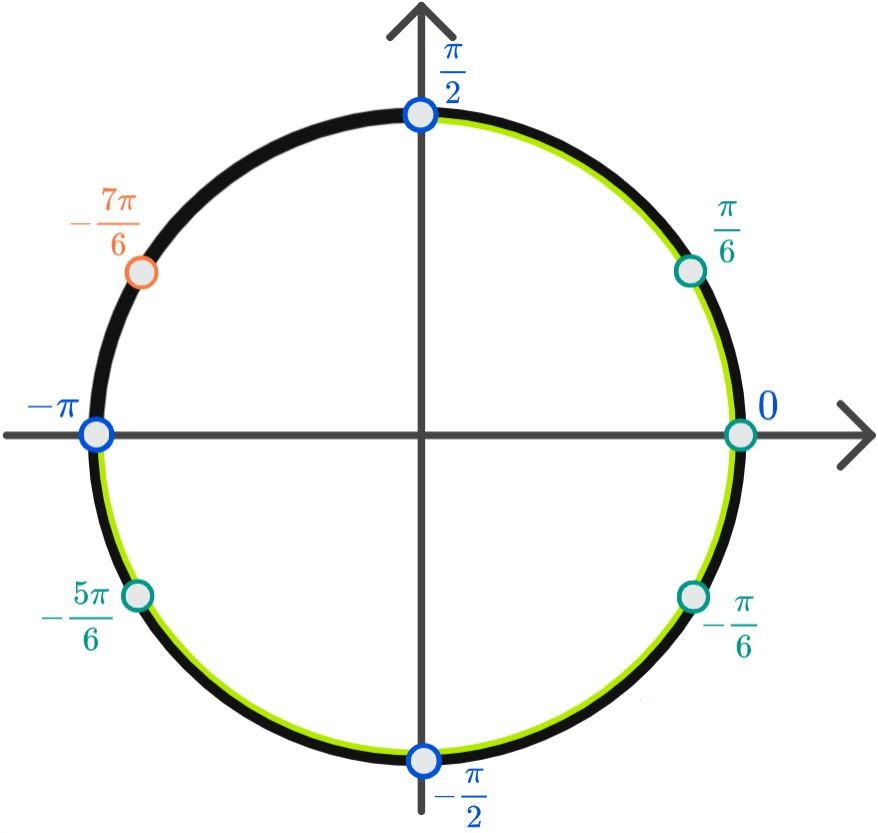
\includegraphics[width=\linewidth]{sol52}\end{figure}\end{minipage}
\end{minipage}}
{a) Решениями являются $x = \pm\frac{\pi}{6} + \pi n,\; n\in\mathbb{Z}$.\\
~\hspace*{1.65cm} b) На отрезке $\left[-\pi;\, \frac{\pi}{2}\right]$ находятся три корня:  $x = -\frac{5\pi}{6}$, $x = -\frac{\pi}{6}$ и $x = \frac{\pi}{6}$.}{Сделать замену, свести к решению простейших уравнений.}
\end{problem}

\begin{problem}{Методы решения тригонометрических уравнений-1.}{10.3.6}{9D}{(лёгкая)}
{a) Решить уравнение $6\cos^{2} x + 5\sqrt{2}\sin x + 2 = 0$.
\\b) Найти все корни этого уравнения, принадлежащие отрезку $\displaystyle \left[\pi;\, \frac{5\pi}{2}\right]$.}
{Используем основное тригонометрическое тождество: $\cos^2 x = 1 - \sin^2 x$, а значит, $6(1 - \sin^2 x) + 5\sqrt{2}\sin x + 2 = 0 \;\Rightarrow\; -6\sin^2 x + 5\sqrt{2}\sin x + 8 = 0$.\\
Сделаем замену $t = \sin x$: получаем квадратное уравнение $\,-6t^2 + 5\sqrt{2}t + 8 = 0$.\\
Решаем через дискриминант: $D = (5\sqrt{2})^2 - 4(-6)\cdot8 = 50 + 192 = 242 = 2\cdot121$.\\
$\displaystyle t_{1, 2} = \frac{-5\sqrt{2} \pm 11\sqrt{2}}{-12} \;\Leftrightarrow\; \left[\begin{aligned}
t &= -\frac{\sqrt{2}}{2}\\
t &= \frac{4\sqrt{2}}{3}
\end{aligned}\right. \;\Leftrightarrow\; \left[\begin{aligned}
\sin x &= -\frac{\sqrt{2}}{2}\\
\sin x &= \frac{4\sqrt{2}}{3}
\end{aligned}\right. \;\Leftrightarrow\; \left[\begin{aligned}
x &= -\frac{\pi}{4} + 2\pi n,\, n \in \mathbb{Z}\\
x &= \frac{5\pi}{4} + 2\pi n,\, n \in \mathbb{Z}\\
x &\in \varnothing
\end{aligned}\right.$\\
(Уравнение $\sin x = \frac{4\sqrt{2}}{3}$ не имеет корней, поскольку $\frac{4\sqrt{2}}{3} > 1$). Таким образом, \\ решениями уравнения являются $x = -\frac{\pi}{4} + 2\pi n$, $n \in \mathbb{Z}\,$ и
$\,x = \frac{5\pi}{4} + 2\pi n$, $n \in \mathbb{Z}$.\smallskip\\
Выберем корни уравнения, лежащие на отрезке $\left[\pi;\, \frac{5\pi}{2}\right]$. Данный отрезок содержит III, IV, и I четверть целиком. Поэтому корни $x = \frac{5\pi}{4}\,$ и $\,x = -\frac{\pi}{4} + 2\pi = \frac{7\pi}{4}$ лежат на данном отрезке, а других нет.}
{a) Решениями являются $x = -\frac{\pi}{4} + 2\pi n$, $n \in \mathbb{Z}\,$ и
$\,x = \frac{5\pi}{4} + 2\pi n$, $n \in \mathbb{Z}$.\smallskip\\
~\hspace*{1.65cm} b) На отрезке $\left[\pi;\, \frac{5\pi}{2}\right]$ лежат корни $\frac{5\pi}{4}$ и $\frac{7\pi}{4}$.}{Данное уравнение решается заменой.}
\end{problem}

\begin{problem}{Методы решения тригонометрических уравнений-1.}{10.3.6}{9D}{(лёгкая)}
{a) Решить уравнение $4\cos^{4} x - 4\cos^{2} x + 1 = 0$.
\\b) Найти все корни этого уравнения, принадлежащие промежутку $[-2\pi; -\pi]$.}
{Нетрудно заметить, что в данном уравнении несколько раз встречается выражение $\cos^2 x$, а других вхождений $x$ нет. Делаем замену: $t = \cos^2 x \;\Rightarrow\; 4t^2 - 4t + 1 = 0 \; \Rightarrow\; (2t - 1)^2 = 0 \;\Rightarrow\; t = \frac12$. Раз мы нашли $t$, делаем обратную замену: $\cos^2 x = \frac12 \;\Rightarrow\; \cos x = \pm \sqrt{\frac12} = \pm \sqrt{\frac24} = \pm\frac{\sqrt{2}}{2}$, поэтому либо $\cos x = \frac{\sqrt{2}}{2}$, либо $\cos x = -\frac{\sqrt{2}}{2}$. Решаем по очереди: $\cos x = \frac{\sqrt{2}}{2} \;\Rightarrow\; x = \pm\frac{\pi}{4} + 2\pi n$, $n \in \mathbb{Z}$. $\cos x = -\frac{\sqrt{2}}{2} \;\Rightarrow\; x = \pm\frac{3\pi}{4} + 2\pi n$, $n \in \mathbb{Z}$. Все эти решения можно объединить и записать так: $x = \frac{\pi}{4} + \frac{\pi k}{2}$, $k \in \mathbb{Z}$. На отрезке $[-2\pi; -\pi]$ находятся решения $x = -\frac{7\pi}{4}$ и $x = -\frac{5\pi}{4}$, других нет ($-\frac{9\pi}{4} < -2\pi$, $-\frac{3\pi}{4} > -\pi$).}
{Уравнение $4\cos^{4} x - 4\cos^{2} x + 1 = 0$ имеет решения $x = \frac{\pi}{4} + \frac{\pi k}{2}$, $k \in \mathbb{Z}$.\\ На отрезке $[-2\pi; -\pi]$ находятся два корня: $x = -\frac{7\pi}{4}\,$ и $\,x = -\frac{5\pi}{4}$.}{Здесь полезно сделать замену.}
\end{problem}

\begin{problem}{Методы решения тригонометрических уравнений-1.}{10.3.6}{9D}{(лёгкая)}
{a) Решить уравнение $\,\displaystyle \tg^{2} x + (1 + \sqrt{3})\tg x + \sqrt{3} = 0$.
\\b) Указать корни этого уравнения, принадлежащие отрезку $\displaystyle \left[\frac{5\pi}{2}; 4\pi\right]$.}
{a) Сделаем замену $t = \tg x$. Получаем квадратное уравнение на $t$ с иррациональными коэффициентами: $t^2 + (1 + \sqrt{3})t + \sqrt{3} = 0$. Решаем уравнение через дискриминант: $D = (1 + \sqrt{3})^2 - 4\sqrt{3} = (\sqrt{3} - 1)^2 \:\Rightarrow\: t = \frac{-(1 + \sqrt{3}) \pm (\sqrt{3} - 1)}{2} = -\sqrt{3};\,-1$.\\
Таким образом, $\tg x = -\sqrt{3}$ или $\tg x = -1$. Оба значения являются табличными, получаем, что $x = -\frac{\pi}{3} + \pi n$, $n \in \mathbb{Z}$, или $x = -\frac{\pi}{4} + \pi n$, $n \in \mathbb{Z}$.\smallskip\\
b) Выясним, какие из корней находятся на отрезке $\left[\frac{5\pi}{2}; 4\pi\right]$. Этот отрезок полностью охватывает II, III, и IV четверть. Наши корни лежат во второй и четвёртой четвертях (тангенс отрицателен). Выясним, какие корни попадают в этот отрезок: это $x = -\frac{\pi}{3} \!+\! 3\pi = \frac{8\pi}{3}$, $\,x = -\frac{\pi}{4} \!+\! 3\pi = \frac{11\pi}{4}$ и $\,x = -\frac{\pi}{3} \!+\! 4\pi = \frac{11\pi}{3}$, $\,x = -\frac{\pi}{4} \!+\! 4\pi = \frac{15\pi}{4}$.\\ Других корней, попадающих в этот промежуток, нет.}
{a) $x = -\frac{\pi}{3} + \pi n$, $n \in \mathbb{Z}$, или $x = -\frac{\pi}{4} + \pi n$, $n \in \mathbb{Z}$.\\ b) На выделенном отрезке находится четыре корня: $x = \frac{8\pi}{3}$ и $x = \frac{11\pi}{4}$ во второй четверти и $x = \frac{11\pi}{3}$ и $x = \frac{15\pi}{4}$ в четвёртой четверти.}{Для решения уравнения нужно сделать замену.\\ Для выбора корней можно выписать их в порядке возрастания.}
\end{problem}

\end{document}